\section{Definition of the signal regions}
\label{sec:sigregion}

We define signal regions to look for possible
new physics contributions by adding the requirement of large MET to the preselection. 
Our choice of MET requirements to define the signal regions is driven by the 
MET distributions expected from $Z$ and $t\bar{t}$ MC with the preselection applied, 
as shown in Fig.~\ref{fig:metdist}. The equivalent luminosity of the $Z$ MC is 
approximately 834 pb$^{-1}$, and that of the \ttbar sample is approximately 6.8 fb$^{-1}$.

\begin{figure}[tbh]
  \begin{center}
	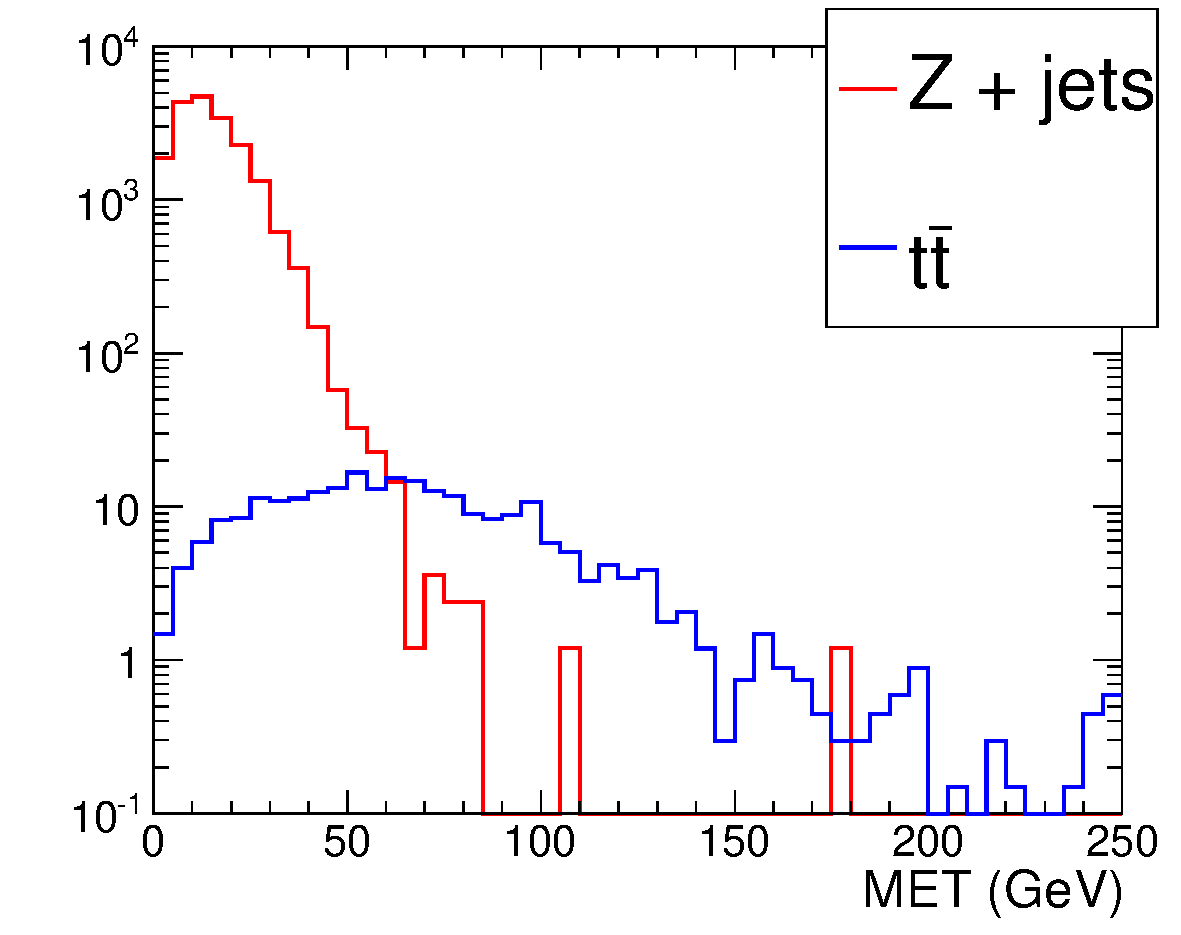
\includegraphics[width=0.75\linewidth]{plots/met_ttbar_Z.pdf}
	\caption{
	  \label{fig:metdist}\protect 
	  Distributions of MET in $Z$ and $t\bar{t}$ MC normalized to 1~fb$^{-1}$.}
  \end{center}
\end{figure}


In addition to our two signal discussed below regions, 
we use the regions MET $>$ 30 GeV and MET $>$ 60 GeV
as very loose signal regions. The mass distributions for these regions are shown in
figures \ref{fig:dilmass30} and \ref{fig:dilmass60}.
For all mass plots in this section, backgrounds from single top 
and $W$+jets are omitted since they are negligible.

\begin{figure}[hbt]
  \begin{center}
	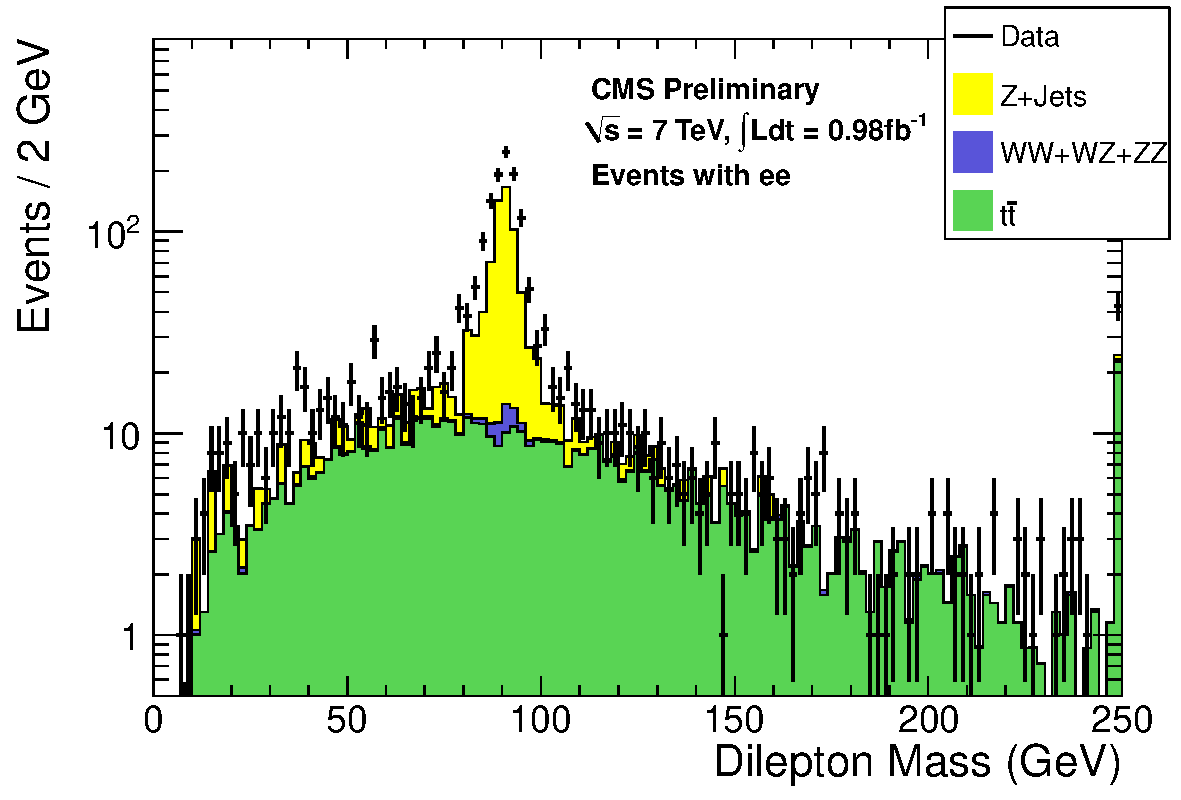
\includegraphics[width=0.48\linewidth]{plots/hdilmass_pfmet30_ee_allj.pdf}
	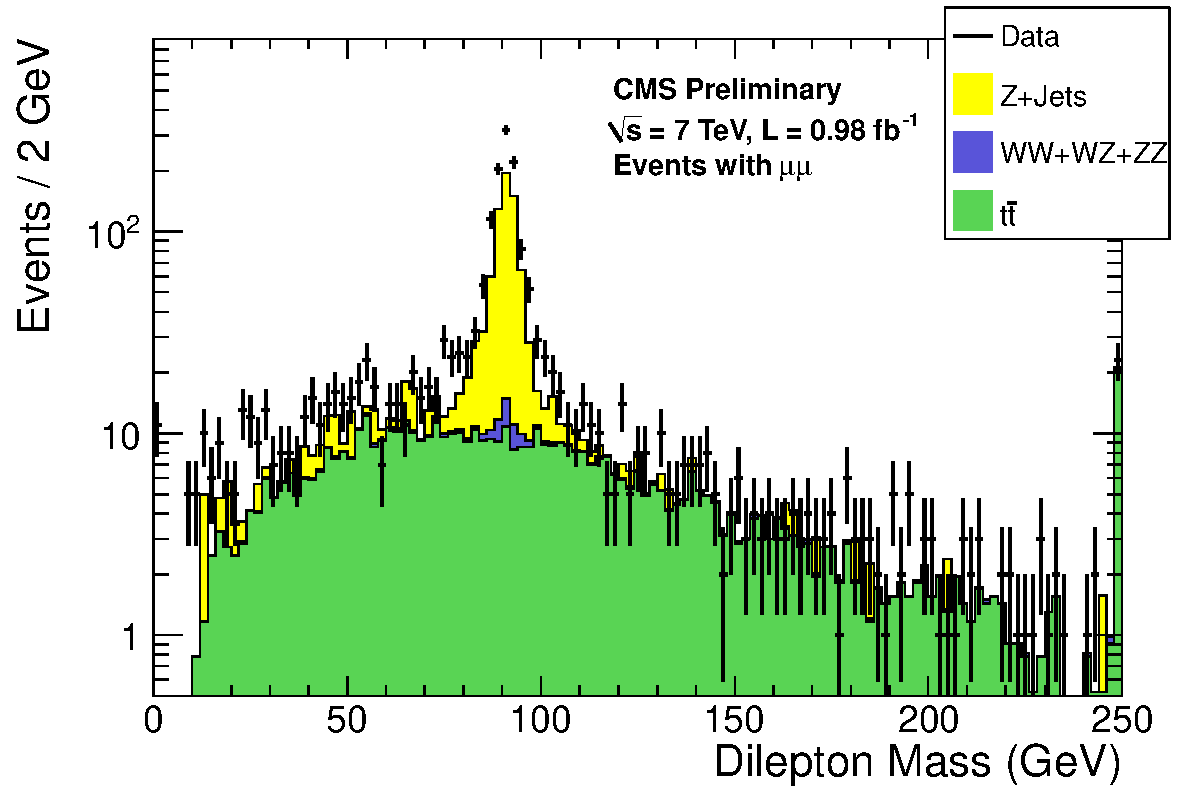
\includegraphics[width=0.48\linewidth]{plots/hdilmass_pfmet30_mm_allj.pdf}
	\caption{
	  \label{fig:dilmass30}\protect 
	  Dilepton mass distribution for events passing the pre-selection 
	  and MET $>$ 30 GeV for \lumi\ in the $ee$ (left) and $\mu\mu$ (right) final states. 
	  Note that because the MC does not model instrumental MET tails well, the MC yield for this MET cut is underestimated.
	  %Backgrounds from single top and $W$+jets are omitted since they are negligible.
	}
  \end{center}
\end{figure}

\begin{figure}[hbt]
  \begin{center}
	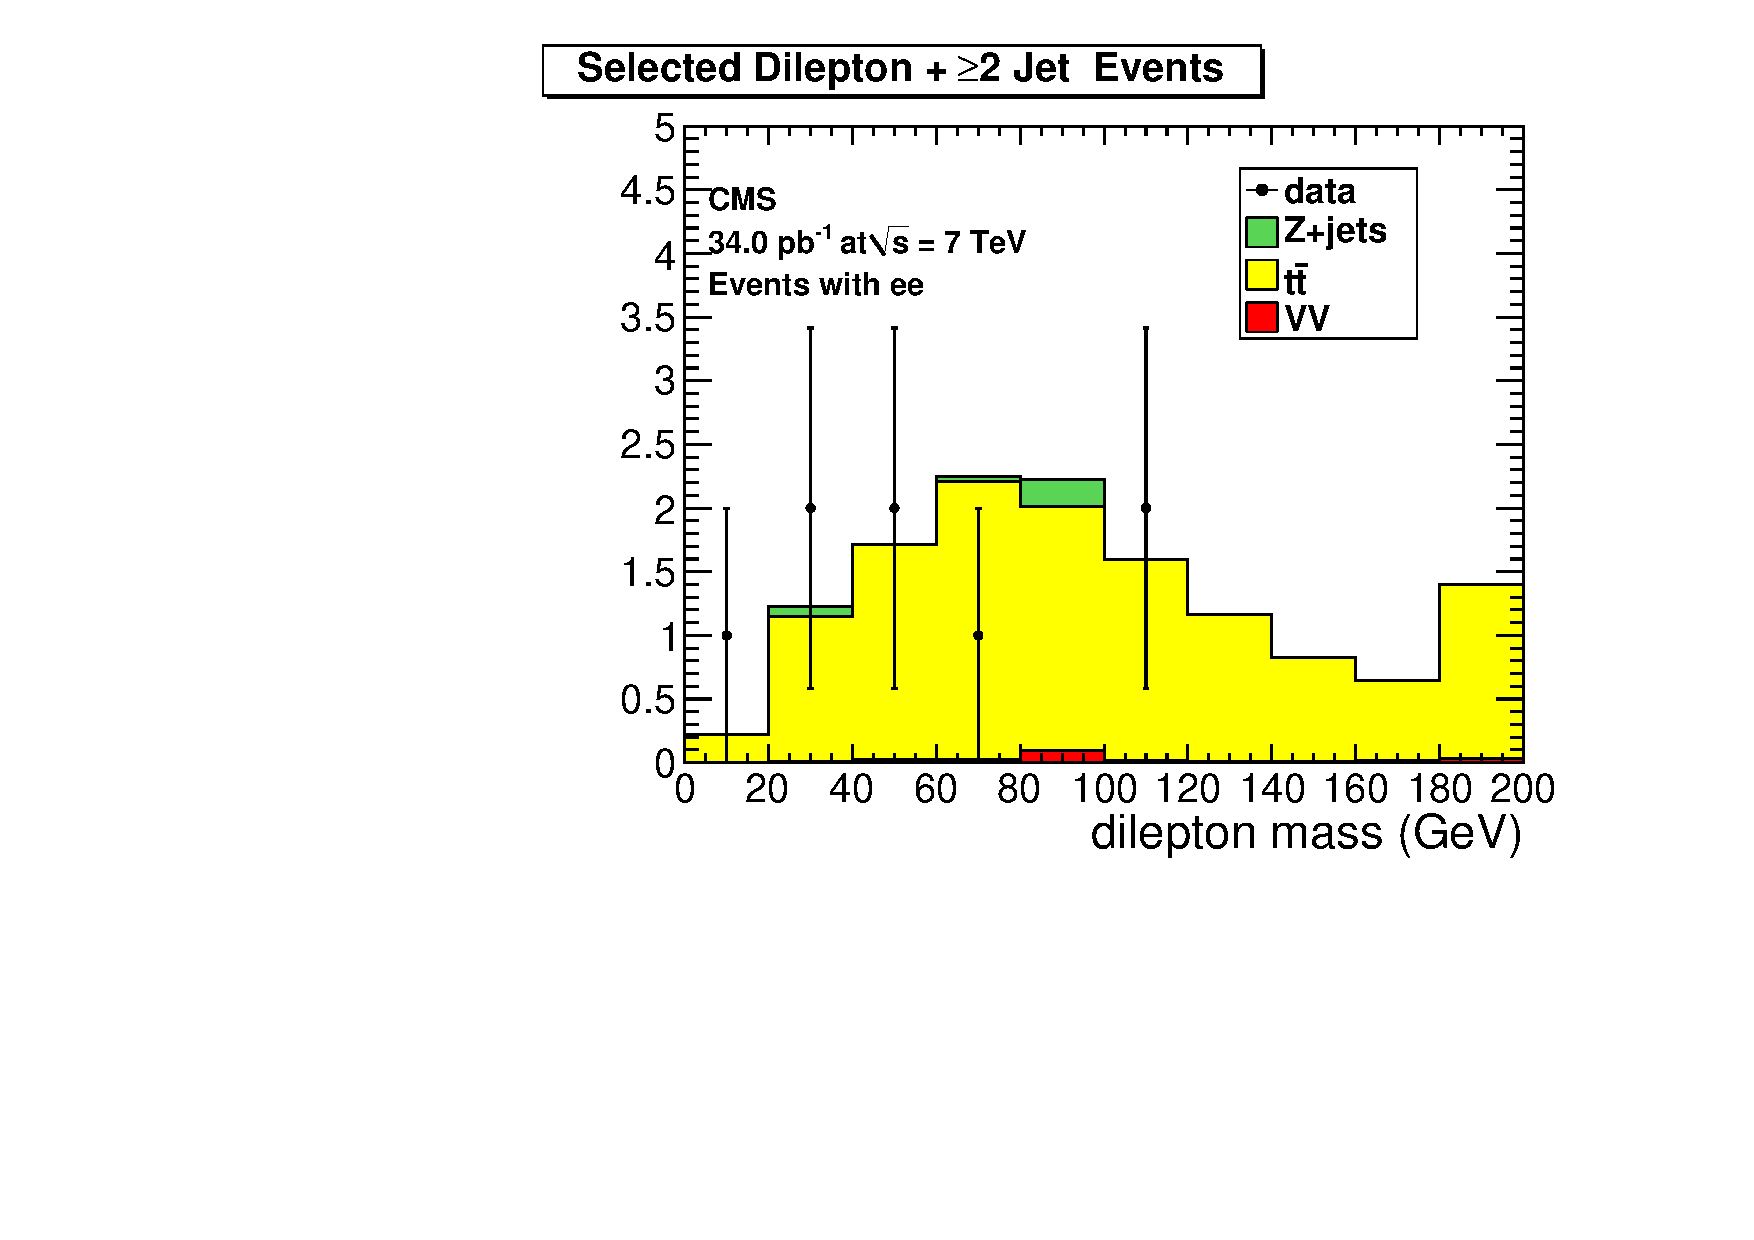
\includegraphics[width=0.48\linewidth]{plots/hdilmass_pfmet60_ee_allj.pdf}
	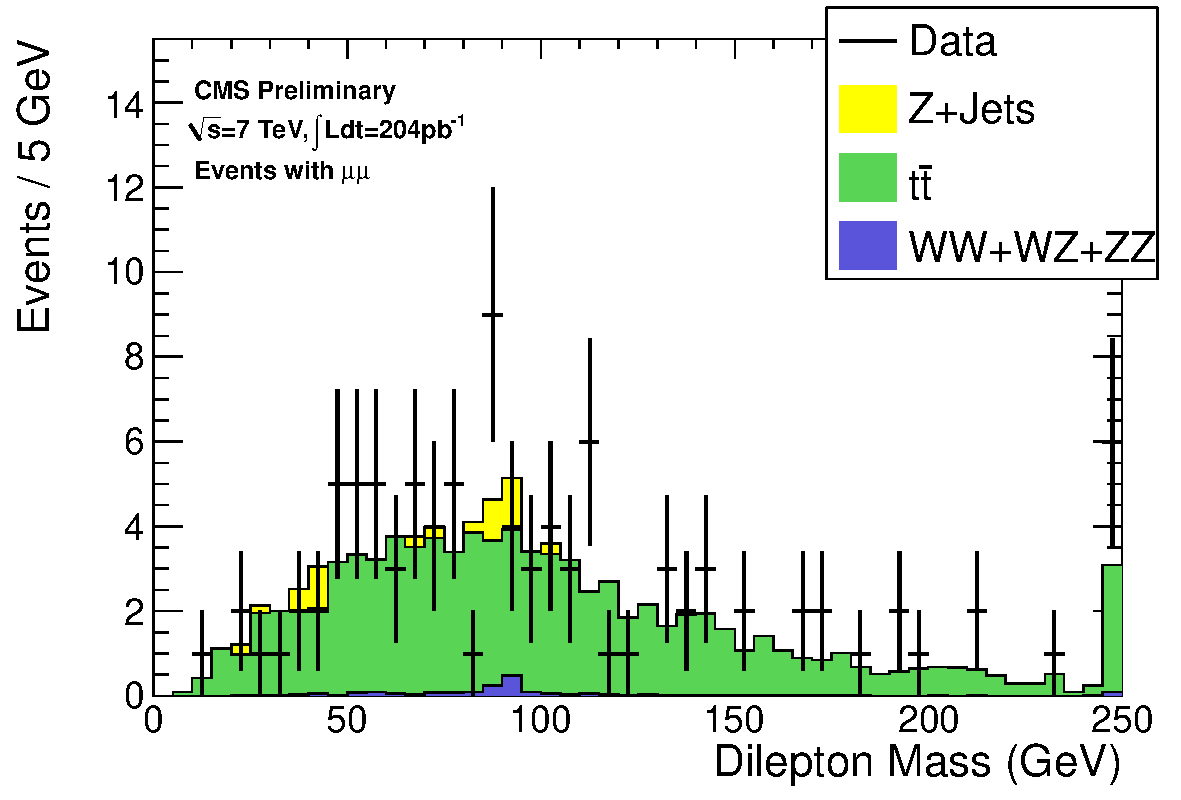
\includegraphics[width=0.48\linewidth]{plots/hdilmass_pfmet60_mm_allj.pdf}
	\caption{
	  \label{fig:dilmass60}\protect 
	  Dilepton mass distribution for events passing the pre-selection 
	  and MET $>$ 60 GeV for \lumi\ in the $ee$ (left) and $\mu\mu$ (right) final states. 
	  %Backgrounds from single top and $W$+jets are omitted since they are negligible.
	}
  \end{center}
\end{figure}


We define two signal regions for our search:

\begin{itemize}
\item MET $>$ \signalmetl~GeV (loose signal region):
  %In this region of MET there is a contribution from the tail of the MET distribution 
  In this region of MET there is a small contribution from the tail of the MET distribution 
  in \Z plus jets events. 
  %There is also a contribution from \ttbar events where the leptons happen to be in the \Z 
  The bulk of the events in this region are from \ttbar events where the leptons happen to be in the \Z 
  mass window.

  %We expect the MC simulation to do a good job on the second source, as it is well within the 
  %bulk of the \ttbar phase space. However, for the first we must rely on data driven procedures. 

  The MC and data yields for this signal region are given in Table~\ref{sigyieldtableloose} and the dilepton
  mass distributions are shown in Fig.~\ref{fig:dilmass100}.

  %until i fix the lumi, don't know what signal events i have

  More information on the data events in this signal region is given in Tables \ref{sig60eventsee}
  and \ref{sig60eventsmm} in appendix \ref{sec:sigevts}.
  %and information 
  %on the muons in these events is given in Table~\ref{sig60muons}.

\item MET $>$ \signalmett~GeV (tight signal region):
  %Though this wording worked when we had a fixed lumi, it doesn't work when we don't know how much we'll get by the end of the year. Just reword.
  This signal region was selected by picking a region where the SM 
  % prediction for the dataset we have is  $\approx$ 1 event. 
  expectation is very low.
  At this kinematical region the dominant background contribution is expected to be from \ttbar.

  The MC and data yields for this signal region are given in Table~\ref{sigyieldtabletight}.

\end{itemize}

In the two signal regions above, the dominant background is \ttbar. 
However, it is still essential to have a data driven estimation of the \Z contribution
in the signal regions to demonstrate that we understand our background composition (see section \ref{sec:templates}).
This is important both in case when an excess is observed or when placing a limit on new physics.

%It's right below this, so why bother -- just put the reference in above
%The data driven technique used to predict the missing transverse energy accompanying 
%a \Z event is described in Section~\ref{sec:templates}.

To estimate the \ttbar background we will use the opposite flavor subtraction
described in Section~\ref{sec:topbkg}.


\begin{figure}[hbt]
  \begin{center}
	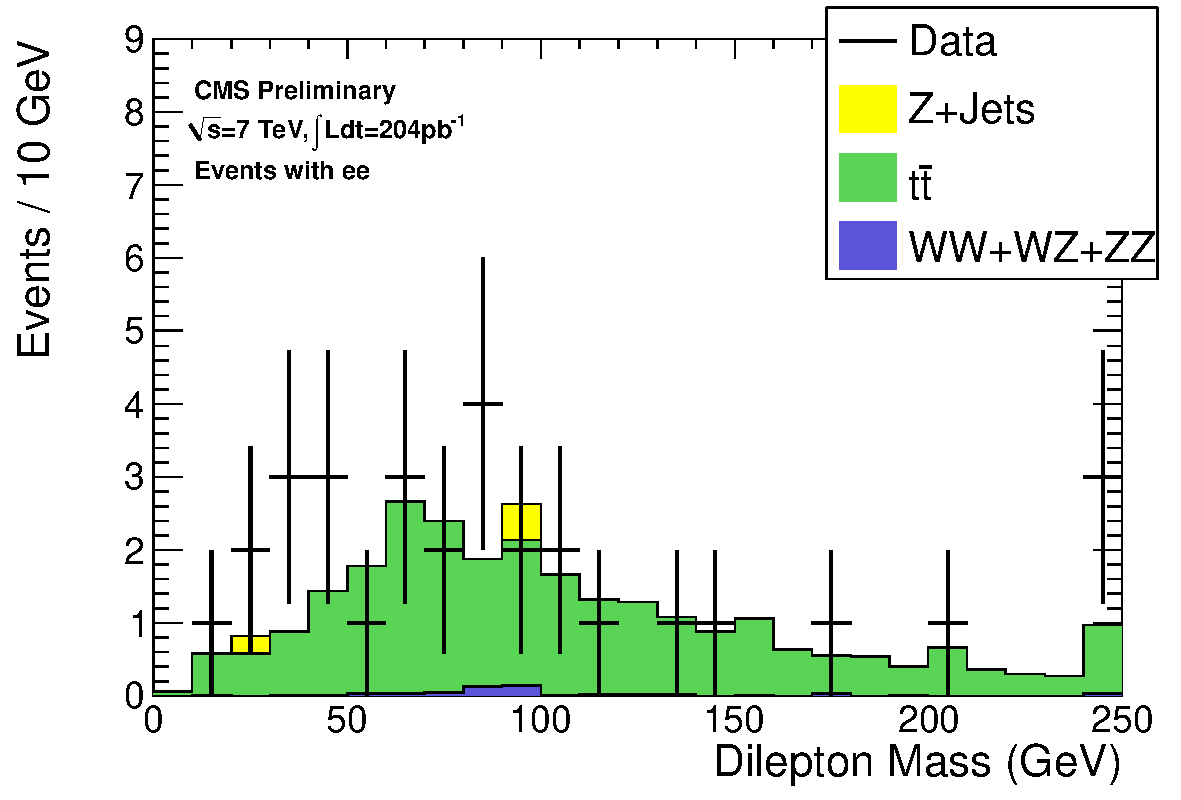
\includegraphics[width=0.48\linewidth]{plots/hdilmass_pfmet100_ee_allj.pdf}
	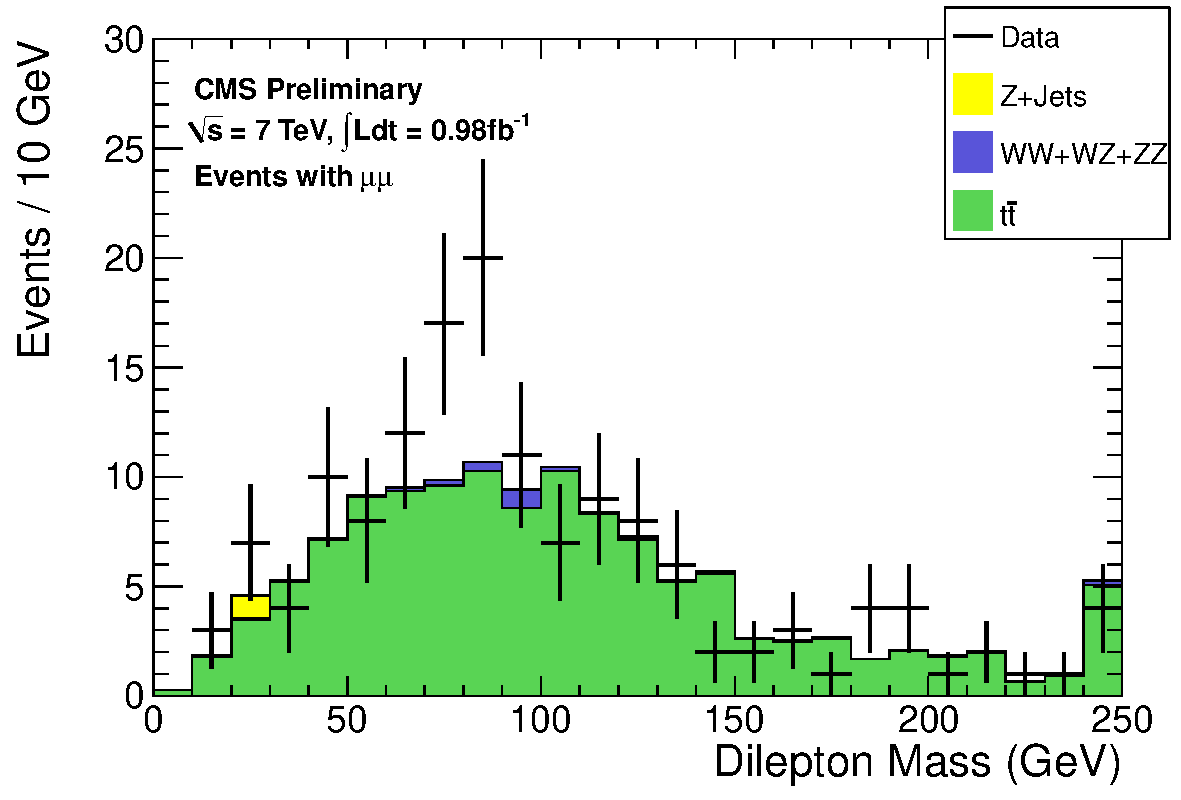
\includegraphics[width=0.48\linewidth]{plots/hdilmass_pfmet100_mm_allj.pdf}
	\caption{
	  \label{fig:dilmass100}\protect 
	  Dilepton mass distribution for events passing the pre-selection 
	  and MET $>$ \signalmetl~GeV for \lumi\ in the $ee$ (left) and $\mu\mu$ (right) final states. 
	  %Backgrounds from single top and $W$+jets are omitted since they are negligible.
	}
  \end{center}
\end{figure}


\begin{table}[htb]
\begin{center}
\caption{\label{sigyieldtableloose} Data and Monte Carlo yields for the loose signal region MET $>$ \signalmetl~GeV  for \lumi.}
\begin{tabular}{lccccc}
\hline
     Sample   &                $ee$   &            $\mu\mu$   &              $e\mu$   &                 tot  \\
\hline
       Z+Jets &   2.34 $\pm$   1.65  &    0.00 $\pm$   0.00  &    0.00 $\pm$   0.00  &    2.34 $\pm$   1.65 \\ 
     \ttbar   &  17.77 $\pm$   1.60  &   18.59 $\pm$   1.55  &   38.42 $\pm$   2.30  &   74.78 $\pm$   3.20 \\ 
        WJets &   0.00 $\pm$   0.00  &    0.00 $\pm$   0.00  &    0.00 $\pm$   0.00  &    0.00 $\pm$   0.00 \\ 
           WW &   0.12 $\pm$   0.07  &    0.25 $\pm$   0.10  &    0.46 $\pm$   0.13  &    0.83 $\pm$   0.18 \\ 
           WZ &   0.68 $\pm$   0.08  &    0.55 $\pm$   0.06  &    0.02 $\pm$   0.01  &    1.25 $\pm$   0.10 \\ 
           ZZ &   0.41 $\pm$   0.03  &    0.41 $\pm$   0.03  &    0.00 $\pm$   0.00  &    0.83 $\pm$   0.05 \\ 
   Single Top &   0.49 $\pm$   0.10  &    0.57 $\pm$   0.10  &    1.16 $\pm$   0.15  &    2.22 $\pm$   0.21 \\ 
\hline
     Total MC &  21.81 $\pm$   2.31  &   20.38 $\pm$   1.56  &   40.06 $\pm$   2.31  &   82.25 $\pm$   3.62 \\ 
\hline
         Data &     25  &      32  &      49  &     106 \\ 
\hline
          LM4 &  10.38 $\pm$   0.36  &    9.68 $\pm$   0.33  &    1.57 $\pm$   0.14  &   21.64 $\pm$   0.51 \\ 
          LM8 &   4.27 $\pm$   0.15  &    4.42 $\pm$   0.15  &    1.58 $\pm$   0.09  &   10.26 $\pm$   0.23 \\ 
\hline
\end{tabular}
\end{center}
\end{table}


\begin{table}[htb]
\begin{center}
  \caption{
	\label{sigyieldtabletight} 
	Data and Monte Carlo yields for the tight signal region MET $>$ \signalmett~GeV  for \lumi.}
\begin{tabular}{lccccc}
\hline
     Sample   &                $ee$   &            $\mu\mu$   &              $e\mu$   &                 tot  \\
\hline
       Z+Jets &   0.00 $\pm$   0.00  &    0.00 $\pm$   0.00  &    0.00 $\pm$   0.00  &    0.00 $\pm$   0.00 \\ 
     \ttbar   &   0.87 $\pm$   0.35  &    0.78 $\pm$   0.32  &    2.20 $\pm$   0.55  &    3.84 $\pm$   0.73 \\ 
        WJets &   0.00 $\pm$   0.00  &    0.00 $\pm$   0.00  &    0.00 $\pm$   0.00  &    0.00 $\pm$   0.00 \\ 
           WW &   0.00 $\pm$   0.00  &    0.04 $\pm$   0.04  &    0.04 $\pm$   0.04  &    0.07 $\pm$   0.05 \\ 
           WZ &   0.13 $\pm$   0.03  &    0.09 $\pm$   0.03  &    0.00 $\pm$   0.00  &    0.22 $\pm$   0.04 \\ 
           ZZ &   0.06 $\pm$   0.01  &    0.06 $\pm$   0.01  &    0.00 $\pm$   0.00  &    0.12 $\pm$   0.02 \\ 
   Single Top &   0.00 $\pm$   0.00  &    0.06 $\pm$   0.03  &    0.04 $\pm$   0.03  &    0.10 $\pm$   0.04 \\ 
\hline
     Total MC &   1.05 $\pm$   0.36  &    1.02 $\pm$   0.32  &    2.27 $\pm$   0.55  &    4.35 $\pm$   0.73 \\ 
\hline
         Data &      1  &       3  &       3  &       7 \\ 
\hline
          LM4 &   6.34 $\pm$   0.28  &    5.93 $\pm$   0.26  &    0.87 $\pm$   0.11  &   13.13 $\pm$   0.40 \\ 
          LM8 &   2.51 $\pm$   0.12  &    2.49 $\pm$   0.11  &    1.03 $\pm$   0.08  &    6.03 $\pm$   0.17 \\ 
\hline
\end{tabular}
\end{center}
\end{table}






%%%%%%%%%%%%%%%%%%%%%%%%%%%%%%%%%%%%%%%%%
%204/pb
%%%%%%%%%%%%%%%%%%%%%%%%%%%%%%%%%%%%%%%%%

\begin{comment}
       Z+Jets &  0.489 $\pm$  0.346  &   0.000 $\pm$  0.000  &   0.000 $\pm$  0.000  &   0.489 $\pm$  0.346 \\ 
       \ttbar &  3.714 $\pm$  0.335  &   4.317 $\pm$  0.361  &   8.454 $\pm$  0.505  &  16.485 $\pm$  0.705 \\ 
        WJets &  0.000 $\pm$  0.000  &   0.000 $\pm$  0.000  &   0.000 $\pm$  0.000  &   0.000 $\pm$  0.000 \\ 
           WW &  0.025 $\pm$  0.014  &   0.058 $\pm$  0.022  &   0.100 $\pm$  0.029  &   0.184 $\pm$  0.039 \\ 
           WZ &  0.155 $\pm$  0.017  &   0.144 $\pm$  0.016  &   0.004 $\pm$  0.002  &   0.303 $\pm$  0.023 \\ 
           ZZ &  0.088 $\pm$  0.007  &   0.096 $\pm$  0.007  &   0.000 $\pm$  0.000  &   0.184 $\pm$  0.010 \\ 
   Single Top &  0.102 $\pm$  0.021  &   0.133 $\pm$  0.024  &   0.256 $\pm$  0.034  &   0.490 $\pm$  0.047 \\ 
\hline
     Total MC &  4.572 $\pm$  0.482  &   4.749 $\pm$  0.363  &   8.814 $\pm$  0.507  &  18.134 $\pm$  0.788 \\ 
\hline
         Data &      7               &       7               &      12               &      26 \\ 
\hline
          LM4 &  2.171 $\pm$  0.075  &   2.248 $\pm$  0.076  &   0.345 $\pm$  0.032  &   4.764 $\pm$  0.112 \\ 
          LM8 &  0.892 $\pm$  0.031  &   1.026 $\pm$  0.034  &   0.347 $\pm$  0.021  &   2.265 $\pm$  0.051 \\ 

%LO
%          LM4 &  1.522 $\pm$  0.052  &   1.603 $\pm$  0.053  &   0.232 $\pm$  0.020  &   3.356 $\pm$  0.077 \\ 
%          LM8 &  0.597 $\pm$  0.020  &   0.686 $\pm$  0.022  &   0.219 $\pm$  0.012  &   1.502 $\pm$  0.032 \\ 




       Z+Jets &  0.000 $\pm$  0.000  &   0.000 $\pm$  0.000  &   0.000 $\pm$  0.000  &   0.000 $\pm$  0.000 \\ 
     \ttbar   &  0.181 $\pm$  0.074  &   0.181 $\pm$  0.074  &   0.483 $\pm$  0.121  &   0.845 $\pm$  0.160 \\ 
        WJets &  0.000 $\pm$  0.000  &   0.000 $\pm$  0.000  &   0.000 $\pm$  0.000  &   0.000 $\pm$  0.000 \\ 
           WW &  0.000 $\pm$  0.000  &   0.008 $\pm$  0.008  &   0.008 $\pm$  0.008  &   0.017 $\pm$  0.012 \\ 
           WZ &  0.025 $\pm$  0.007  &   0.021 $\pm$  0.006  &   0.000 $\pm$  0.000  &   0.046 $\pm$  0.009 \\ 
           ZZ &  0.013 $\pm$  0.003  &   0.013 $\pm$  0.003  &   0.000 $\pm$  0.000  &   0.026 $\pm$  0.004 \\ 
   Single Top &  0.000 $\pm$  0.000  &   0.013 $\pm$  0.008  &   0.009 $\pm$  0.006  &   0.022 $\pm$  0.010 \\ 
\hline
     Total MC &  0.219 $\pm$  0.074  &   0.237 $\pm$  0.075  &   0.500 $\pm$  0.121  &   0.956 $\pm$  0.161 \\ 
\hline
         Data &      0               &       2               &       2               &       4 \\ 
\hline
          LM4 &  1.324 $\pm$  0.059  &   1.377 $\pm$  0.060  &   0.191 $\pm$  0.023  &   2.892 $\pm$  0.087 \\ 
          LM8 &  0.524 $\pm$  0.024  &   0.578 $\pm$  0.025  &   0.228 $\pm$  0.017  &   1.330 $\pm$  0.039 \\ 

%LO
%          LM4 &  0.922 $\pm$  0.040  &   0.969 $\pm$  0.041  &   0.128 $\pm$  0.015  &   2.019 $\pm$  0.060 \\ 
%          LM8 &  0.345 $\pm$  0.015  &   0.387 $\pm$  0.016  &   0.144 $\pm$  0.010  &   0.876 $\pm$  0.024 \\ 

\end{comment}

